\documentclass{article}
\usepackage[utf8]{inputenc} %tildes y caracteres especiales
%\usepackage[spanish]{babel} 
\usepackage{amsmath, amssymb}
\usepackage{geometry}
\usepackage{fancyhdr}
\usepackage{enumitem}
\usepackage{titlesec}
\usepackage{graphicx}
\usepackage{physics}
\usepackage{xcolor}
\usepackage{ragged2e}

\usepackage{tikz}
\usepackage{pgfplots}
\pgfplotsset{compat=1.18}
\usepackage{tikz-3dplot} % Permite coordenadas 3D

\allowdisplaybreaks
\setlength{\parindent}{0pt}

\geometry{
  top=2.54cm,
  bottom=2.54cm,
  left=2.54cm,
  right=2.54cm
} %MARGENES APA

% Estilo personalizado
\pagestyle{fancy}
\fancyhf{}
\rhead{Taller No. 3-Teoría Electromagnética}
\rfoot{ \thepage}
\renewcommand{\footrulewidth}{0.4pt} % línea sobre pie de página (default: 0pt → invisible)

\newcommand{\problema}[2]{%
  \vspace{0.5cm}
  {\noindent\textbf{Problema #1} #2} 
  \noindent 
}

% Redefinir sección: texto normal, sin espacio extra
\titleformat{\section}
  {\normalfont}       % Estilo del título (normal, sin negrita)
  {\thesection}       % Numeración (ej. 1, 2, 3...)
  {1em}               % Espacio entre número y título
  {}                  % Código antes del título (vacío)

%--------------------------------------------------------------

\begin{document}
\begin{titlepage}
        \begin{center}
            \LARGE \textbf{Taller No. 3\\Teoría Electromagnética}
            \vfill
            \large

            Karen Alejandra Freire Rosero\\
            Sonier Andrés Ortiz Castelblanco\\
            Sarah Isabel Tejada García\\
            Santiago Alejandro Pérez Ramos
            \vfill
            \textbf{Asignatura:} Teoría Electromagnética\\
            \textbf{Profesor:} Servio Tulio Pérez Merchancano, Ph.D\\
            \vfill
            Universidad del Cauca\\
            Facultad de Ciencias Naturales, Exactas y de la Educación\\
            Departamento de Física\\
            Popayán, Cauca\\
            2025
        \end{center}
\end{titlepage}

\section*{\problema{2.20}{Uno de los siguientes es un campo electrostático imposible. ¿Cuál?}}

\begin{itemize}
    \item[(a)] \( \vec{E} = k(xy \, \hat{x} + 2yz \, \hat{y} + 3xz \, \hat{z}) \)
    \item[(b)] \( \vec{E} = k(y^2 \, \hat{x} + (2xy + z^2) \, \hat{y} + 2yz \, \hat{z}) \)
\end{itemize}

Aquí k es una constante con las unidades apropiadas. Para la posible, halla el potencial, utilizando el origen como punto de referencia.
Comprueba tu respuesta calculando \(\nabla V\)  [Pista: Debes seleccionar una trayectoria específica para integrar. No importa qué camino elijas, ya que la respuesta
es independiente del camino, pero simplemente no puedes integrar a menos que tengas un camino definido en mente].

\subsubsection*{Solución:}
Para un campo electrostático sea físicamente posible este debe ser conservativo, esto es: 

\[
   \quad \nabla \times \vec{E} = \vec{0}
\]

Por lo tanto se procede a realizar el cálculo del rotacional de $\vec{E}$.

\subsubsection*{Caso (a):}
$\vec{E}_{1} = k(xy, 2yz, 3xz)$

\[
\vec{\nabla} \times \vec{E}_{1} = k
\begin{vmatrix}
\hat{x} & \hat{y} & \hat{z} \\
\partial/\partial x & \partial/\partial y & \partial/\partial z \\
xy & 2yz & 3xz
\end{vmatrix}
\]

\begin{align*}
  \curl{\vec{E}_{1}} &= k [(0-2y)\hat{x} + (0-3z)\hat{y} + (0-x)\hat{z}] \\
  \curl{\vec{E}_{1}} &= k [-2y\hat{x} - 3z\hat{y} - x\hat{z} ] \\
  \curl{\vec{E}_{1}} &\neq 0
\end{align*}

Por lo tanto,$\vec{E}_{1}$ no es conservativo y no es posible que sea un campo electrostático
\subsubsection*{Caso (b):}

$\vec{E}_{2} = k(y^2, 2xy+z^2, 2yz)$

\[
\vec{\nabla} \times \vec{E}_{2} = k
\begin{vmatrix}
\hat{x} & \hat{y} & \hat{z} \\
\partial/\partial x & \partial/\partial y & \partial/\partial z \\
y^2 & 2xy+z^2 & 2yz
\end{vmatrix}
\]

\begin{align*}
  \curl{\vec{E}_{2}} &= k [(0-0)\hat{x} + (0-0)\hat{y} + (0-0)\hat{z}] \\
  \curl{\vec{E}_{2}} &= 0
\end{align*}

Por lo tanto, $\vec{E}_{1}$ es un campo electrostático posible, y se puede encontrar el potencial para este caso.
\newpage
Para ello se definiera un camino de integración (trayectoria) $(0,0,0) \rightarrow (x_{0},0,0) \rightarrow (x_{0},y_{0},0) \rightarrow (x_{0},y_{0},z_{0})$, 
como se puede ver en la figura\ref{Camino_de_integracion}:


\begin{figure}[h]
  \centering
  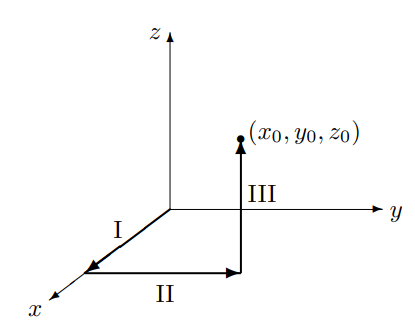
\includegraphics[width=0.4\textwidth]{imagenes/path1.png}
  \caption{\label{Camino_de_integracion}Camino de integración}
  \small Imagen tomada de: *Solutions Manual* de Griffiths, \textit{Introduction to Electrodynamics}.
\end{figure}
El potencial esta dado por:

\begin{align*}
  V &= - \int_{0}^{(x_{0},y_{0},z_{0})} E\cdot\,dl \\
  V &= - \int_{I}^{} E\cdot\,dl - \int_{II}^{} E\cdot\,dl - \int_{III}^{} E\cdot\,dl
\end{align*}
Calculando $E \cdot dl$
\[
  E \cdot dl = k[y^2 dx + (2xy+z^2)dy + 2yz dz]
\]
Camino I$: (0,0,0) \rightarrow (x_{0},0,0); y=z=0 ; dy=dz=0$
\begin{align*}
  E \cdot dl &= k[{(0)}^2 dx + (2x(0)+{(0)}^2)(0) + 2(0)(0)(0)] \\
  E \cdot dl &= 0 \\
  \int_{I}^{} E\cdot\,dl &= 0
\end{align*}

Camino II$: (x_{0},0,0) \rightarrow (x_{0},y_{0},0);x = x_{0} ; z=0 ; dx=dz=0; y:0\rightarrow y_{0}$
\begin{align*}
  E \cdot dl &= k[y^2 (0) + (2x_{0}y+{(0)}^2)dy + 2y(0)(0)] \\
  E \cdot dl &= 2kx_{0}y dy \\
  \int_{I}^{} E\cdot\,dl &= 2kx_{0} \int_{0}^{y_{0}} y\,dy = kx_{0}y_{0}^2
\end{align*}

Camino III$: (x_{0},y_{0},0) \rightarrow (x_{0},y_{0},z_{0}); x = x_{0};y = y_{0} ; dx=dy=0; z:0\rightarrow z_{0}$
\begin{align*}
  E \cdot dl &= k[y_{0}^2 (0) + (2x_{0}y_{0}+z^2)(0) + 2y_{0}zdz] \\
  E \cdot dl &= 2ky_{0}z dz \\
  \int_{I}^{} E\cdot\,dl &= 2ky_{0} \int_{0}^{z_{0}} z\,dz = ky_{0}z_{0}^2
\end{align*}

Sumando cada una de las contribuciones calculadas se puede obtener el potencial total:
\begin{center}
\fbox{$V(x,y,z)=-k(y^2x+yz^2)$}
\end{center}

Verificamos este resultado calculando el gradiente de modo que obtendremos el campo original, $\vec{E} = -\grad{V}$.
\begin{align*}
  \grad{V} &= \frac{\partial V}{\partial x}\hat{x} +\frac{\partial V}{\partial y}\hat{y} + \frac{\partial V}{\partial z}\hat{z}\\
  \grad{V} &= -k y^2\hat{x} - k(x y+z^2)\hat{y} - k2yz\hat{z}\\
  \grad{V} &= -k[y^2\hat{x} + (2xy+z^2)\hat{y} + 2yz\hat{z}] = -E
\end{align*}

\begin{center}
  \fbox{$E=-k[y^2\hat{x} + (2xy+z^2)\hat{y} + 2yz\hat{z}]$}
\end{center}

\section*{\problema{2.22}{Halle el potencial a una distancia s de un hilo recto infinitamente largo que lleva una carga lineal uniforme $\lambda$.
Calcula el gradiente de tu potencial y comprueba que da el campo correcto.}}

\begin{figure}[h]
  \centering
  \begin{tikzpicture}
  % Ejes
  \draw[-, thick] (0,0) -- (4,0) ;  % Eje x (solo positivo)
  \draw[dashed,->] (4,0) -- (5,0) node[below right] {$x$}; % Línea auxiliar vertical
  
  \draw[<->, thick] (0,-1) -- (0,3) ;    % Eje z (positivo y negativo)
  \draw[dashed,->] (0,3) -- (0,4) node[above left] {$z$};
  \draw (0,2.8) to[out=45,in=180] (0.4,3) 
    node[right] {\scriptsize Alambre infinito con densidad $\lambda$};

  \filldraw[blue] (0,0) circle (2pt) node[below left] {$\mathcal{O}$};

  % Línea desde el origen al punto
  \draw[red, thick,->] (0,0) -- (3.5,0);
  \node[red] at (1.5,-0.2) {$s$}; % Etiqueta de distancia
\end{tikzpicture}
\caption{Alambre recto infinitamente largo}
\end{figure}

Para hallar el potencial a una distancia s del origen ($\mathcal{O}$) se plantea la integral de línea

\[
  \int_{s_{0}}^{s}  \vec{E} \cdot dl 
\]

De modo que $s_{0}$ es el punto de referencia tal que $V(s_{0})=0$ y el $\vec{E}$ es el campo de un alambre recto infinitamente largo con dirección radial $\hat{s}$.

\[
  \vec{E} = \frac{1}{4\pi \epsilon_{0}} \frac{2\lambda}{s} \hat{s}
\]

Calculando la integral tenemos

\[ -\frac{2\lambda}{4\pi \epsilon_{0}} \int_{s_{0}}^{s} \frac{1}{s} ds =  \frac{2\lambda}{4\pi{} \epsilon_{0}} \ln(\frac{s}{s_{0}}) \]
\[ \fbox{$V = -\frac{\lambda}{2\pi{} \epsilon_{0}} \ln(\frac{s}{s_{0}})$} \]

Para comprobar que este resultado sea correcto calculamos el campo eléctrico usando $\vec{E} = -\grad{V}$. 

\begin{align*}
  \grad{V} &= -\frac{\partial V}{\partial s} \hat{s} \\
  \grad{V} &=  -\frac{\lambda}{2\pi \epsilon_{0}} \frac{\partial}{\partial s} \left(\ln(\frac{s}{s_{0}})\right) \hat{s}\\
  \grad{V} &=  -\frac{\lambda}{2\pi \epsilon_{0}} \left( \frac{s_{0}}{s} \frac{1}{s_0} \right) \hat{s}
\end{align*}

\begin{center}
  \fbox{$\vec{E}=-\grad{V}=\frac{\lambda}{2\pi \epsilon_{0}} \left( \frac{1}{s} \right) \hat{s}$}  
\end{center}

\section*{\problema{2.24}{Para la configuración del Prob. 2.16, encuentre la diferencia de potencial entre un punto del eje y un punto del cilindro exterior. Tenga en cuenta que no es necesario comprometerse con un punto de referencia en particular, si utiliza la Ec. 2.22.}}

\begin{figure}[h]
  \centering
  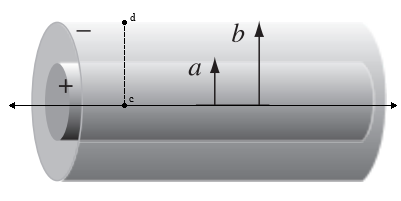
\includegraphics[width=0.5\textwidth]{imagenes/Figure_2.26.png}
  \caption{\label{fig:problema_24}Figura del problema 2.16}
\end{figure}

Para encontrar la diferencia de potencial entre el punto c en el eje de los cilindros y el punto d en la superficie del cilindro de radio b, se plantea la siguiente integral dada por la ecuación 2.22:

\[
  V(d)-V(c) = -\int_{c}^{d} \vec{E} \cdot dl = -\int_{0}^{d} \vec{E} \cdot dl - \int_{0}^{c} \vec{E} \cdot dl
\]

Sin embargo para el punto se se tiene que $V(c)=V(0)=0$, por lo tanto para encontrar la diferencia de potencial solo se calcula la integral desde 0 hasta b

\[ V(d)-V(0) = -\int_{0}^{d} \vec{E} \cdot dl \]

Del problema 2.16 conocemos el campo eléctrico del problema para:
\begin{itemize}
  \item [(a)] $s<a$\
  \begin{align*}
    \vec{E} =\frac{\rho s}{2\epsilon_{0}}\hat{s}
  \end{align*}
  \item [(b)] $a<s<b$
  \begin{align*}
    \vec{E} =\frac{\rho a^2}{2\epsilon_{0} s}\hat{s}
  \end{align*}
\end{itemize}

Por tanto para calcular la integral de $0\rightarrow d$ la dividimos en 2, de $0\rightarrow a$ y $a\rightarrow d$:
\begin{align*}
  -\int_{0}^{d} \vec{E} \cdot dl \ &= -\int_{0}^{a} \vec{E} \cdot dl -\int_{a}^{d} \vec{E} \cdot dl \\
   &= -\int_{0}^{a} \frac{\rho s}{2\epsilon_{0}} ds -\int_{a}^{d} \frac{\rho a^2}{2\epsilon_{0} s} ds \\
   &= -\frac{\rho}{2\epsilon_{0}} \left[ \int_{0}^{a} s ds + a^2 \int_{a}^{d} \frac{1}{s} ds\right]\\
   &= -\frac{\rho}{2\epsilon_{0}} \left[ \frac{s^2}{2} \bigg|_{0}^{a} + a^2 \ln(s) \bigg|_{a}^{b} \right]\\
   &= -\frac{\rho}{2\epsilon_{0}} \left[ \frac{a^2}{2} + a^2 \ln(\frac{b}{a}) \right]\\
   &= -\frac{\rho a^2}{4\epsilon_{0}} \left[ 1 + 2\ln(\frac{b}{a}) \right]\\
\end{align*}

\begin{center}
  \fbox{$V(d)-V(0) = -\frac{\rho a^2}{4\epsilon_{0}} \left[ 1 + 2\ln(\frac{b}{a}) \right]$}
\end{center} 

\end{document}

